\input{../../template.ltx}

\usepackage{graphicx}

\begin{document}

\osuetitle{3}

\section*{Aufgabenstellung}

\textbf{Shared-Integrator}

Schreiben Sie 2 Prozesse zum verteilten Integrieren des bestimmten Integrales 
$$\int^{max}_{min} \frac{x^2}{4}$$

\begin{verbatim}
    SYNOPSIS
        server min max n_per_packet numpackets
        integrate 
\end{verbatim}

Es gibt einen Server-Prozess und beliebige viele Client-Prozesse. 
Der Server teilt den zu integrierenden Bereich in \emph{numpacket} Pakete auf. 
Die Integrier-Prozesse übernehmen jeweils einzelne Pakete integrieren diese und geben das Teilergebnis an den Server zurück. 
Jeder Integrier-Prozess teilt sein Paket wiederum in \emph{n\_per\_packet} Teile auf und verwendet zum Integrieren ein einfaches Riemannsummen-Integral.
$$\int^b_a f(x) = \frac{b-a}n * \sum_{i=1}^{n} f(a+i*\frac{b-a}{n})$$

Danach holen Sie sich ein neues Paket solange bis alles fertig integriert ist. Es kann also durchaus weniger als \emph{numpackets} Integrier-Prozesse geben. Ist alles fertig integriert dann gibt der Server das Ergebnis auf \emph{stdout} aus

\section*{Beispiel {\small($n\_per\_packet=10, numpackets=3$)}}
Das Integral wird in diesem Fall in 3 Pakete zerlegt.
Jedes dieser Pakete wird wiederum in 10 Teile zerlegt von denen dann die Riemannsumme berechnet werden kann.

\begin{center}
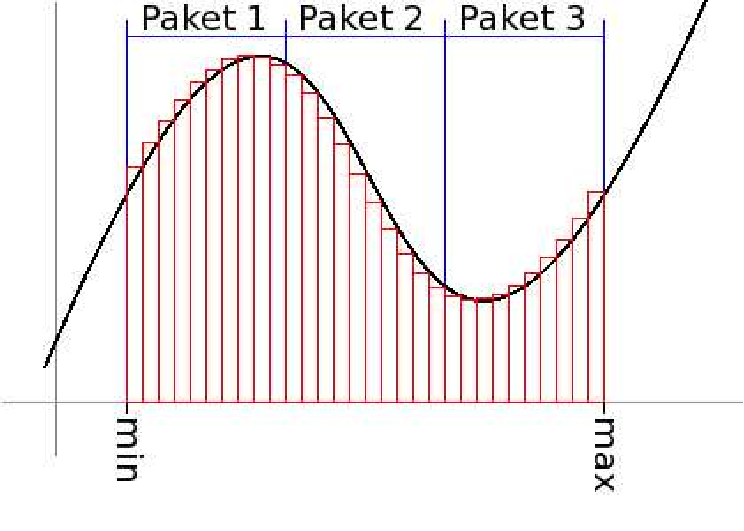
\includegraphics[height=6cm]{integrate.pdf}
\end{center}

\section*{Hinweis}
Die Kommunikation zwischen dem Server-Prozess und den Client-Prozessen soll über einen Shared-Memory gehen. Die Anzahl der Clients ist nicht beschränkt. Sie können zu beliebigen Zeitpunkten gestartet werden und terminieren jeweils wenn kein neues Paket verfügbar ist. Das Integrieren soll beginnen sobald der erste Integrier-Prozess verfügbar ist. Überlegen Sie sich ein geeignetes Synchronisations-Schema für diese Aufgabe.  

\section*{Anleitung}
Schreiben Sie zwei Programme, die die Prozesse mittels einer Client/Server-Struktur realisieren. Achten Sie auf eine saubere Terminierung.

\osueguidelinesthree

\end{document}
